\subsection{Polytopes}
	
	\subsubsection{$\mathcal{H}$-polytopes and $\mathcal{V}$-polytopes}
		The definitions, theorems and lemmas in this section are exclusively taken from \cite{braun2007ehrhart}. 
		
		
		We start by defining convex polytopes. 
		For this we need the definition of convexity and convex hulls. 
		
		\definition{
			A subset $X\subseteq \mathbb{R}^n$ is \emph{convex} if $\theta \textbf{x} + (1-\theta)\textbf{y} \in X$ for every $\textbf{x}, \textbf{y} \in X$ and 
			$\theta \in [0, 1]$.
		}
		
		\definition{
			Given a finite set $Y\subseteq \mathbb{R}^n$, the \emph{convex hull} of $Y$, denoted $\text{conv}\{Y\}$, 
			is the intersection of all convex sets containing $Y$, i.e. 
			\[
			\text{conv}\{Y\} = \left\{ \sum_{\textbf{y}\in Y} a_y \textbf{y} : a_y\in \mathbb{R}_{\geq 0}, \sum_{y \in Y} a_y = 1 \right\}.
			\]
		}
		
		\bigskip
		
		There are two ways to define polytopes;
		these are using halfspaces to define $\mathcal{H}$-polytopes or using vertices 
		to define $\mathcal{V}$-polytopes. 
		We show in Section \ref{proofHVequal} that these definitions are in fact equal. 
		
		\bigskip
		
		We start by defining polytopes using halfspaces. 
		
		\definition{
			A \emph{halfspace} in $\mathbb{R}^n$ is the set of solutions to a linear inequality of the form $\textbf{a} \cdot \textbf{x} \leq b$ 
			where $\textbf{a}\in \mathbb{R}^n$ and $b\in \mathbb{R}$. 
		}
		
		\definition{
			An \emph{affine subspace} $A \subseteq \mathbb{R}^n$ of dimension $d$ is a translate by some fixed $\textbf{y}\in \mathbb{R}^n$ 
			of a $d$-dimensional linear subspace of $\mathbb{R}^n$. 
		}
		
		\definition{
			Given a subset $V \subseteq \mathbb{R}^n$, the \emph{affine span} of $V$, denoted aff$(V)$, is the intersection of all 
			affine subspaces of $\mathbb{R}^n$ containing $V$.
		}
		
		\bigskip		
		
		Halfspaces, affine subspaces and affine spans are linked by the following theorems.
		
		\theorem{
			The affine span of a subset of $\mathbb{R}^n$ is an affine subspace.
		}
		\begin{proof}
			Since affine subspaces are translates of linear subspaces, they satisfy the condition that if 
			$\textbf{x}, \textbf{y} \in A$, $b \in \mathbb{R}$ for some affine subspace $A$, 
			then $b \textbf{x} + \textbf{y} \in A$.
			
			Now, assume there exists $\textbf{x} \in \textbf{y} \in V$. 
			Then for any affine subset containing $V$ there must exist $b \textbf{x} + \textbf{y}$. 
			Thus, $b \textbf{x} + \textbf{y}$ is also in the intersection of all affine subsets containing $V$ 
			and the affine span of $V$ is an affine subset.
		\end{proof}
		
		\theorem{
			The boundary of any halfspace in $\mathbb{R}^n$ is an affine subspace of dimension $n-1$.
		}
		\begin{proof}
			If the boundary contains the vectors $x,y \in \mathbb{R}^n$, it also contains 
			$b \textbf{x} + \textbf{y}$ for some $b \in \mathbb{R}$. 
			This is because any vector in the boundary can be scaled arbitrarily due to the boundary 
			being infinite, and the addition of two vectors in the boundary can only create a vector 
			also in the boundary. Thus, the boundary of a halfspace is an affine subspace.
		
			Obviously, a halfspace in $\mathbb{R}^n$ have dimension $n$. 
			The normal vector $n$ for a halfspace points outwards from the halfspace, orthogonal 
			to the boundary (see Figure \ref{fig:halfspaceandaffinesubspace}).
			The boundary stretches infinitely out in all directions except the direction of the 
			normal vector $n$. 
			Thus, the boundary have a loss of one dimension compared to the halfspace. 
			
			
			We conclude the boundary of a halfspace is an affine set with dimension $n-1$.
		\end{proof}
		\raggedbottom
		
		\emph{We use an example to demonstrate these properties.}
		
		\example{
			The halfspace $H = \{x-y \leq 2:(x,y)\in \mathbb{R}^2\}$ have the boundary $x-y=2$, which is the 1-dimensional affine 
			subspace $A=\{(x,x)+(0,-2):x\in \mathbb{R}\} = \text{aff}(\{(0,-2),(2,0)\})$, 
			see Figure \ref{fig:halfspaceandaffinesubspace}.
		}
		
		\begin{figure}[H]
		\begin{center}
		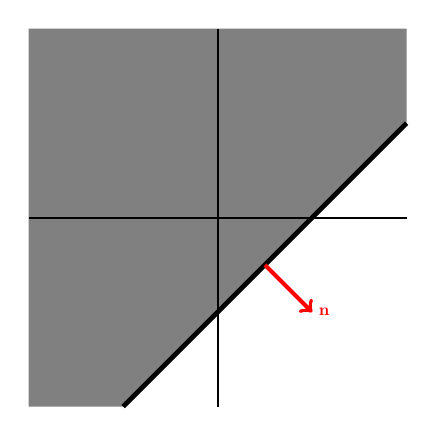
\begin{tikzpicture}[scale=0.6, transform shape]
			\fill[gray] (-2,-4) -- (-4,-4) -- (-4,4) -- (-4,4) -- (4,4) -- (4,2);
			\draw [line width=0.25mm] (-4,0) -- (4,0);
			\draw [line width=0.25mm] (0,-4) -- (0,4);
			\draw [line width=0.6mm] (-2,-4) -- (4,2);
			\coordinate (m) at (1,-1);
			\draw[->, red, line width=0.5mm] (m) -- ++(1,-1) node[right] {$\mathbf n$};
		\end{tikzpicture}
		\end{center}
		\caption{The halfspace $H = \{x-y \leq 2:(x,y)\in \mathbb{R}^2\}$ in gray with its boundary marked using a thick line. Its normal vector $n$ is the red arrow.}
		\label{fig:halfspaceandaffinesubspace}
		\end{figure}
		
		\emph{Finally, we have the definition for the first type of polytope.}
		
		\definition{
			An \emph{$\mathcal{H}$-polytope} of dimension $d$ in $\mathbb{R}^n$ is a bounded intersection $P$ of a finite number of 
			halfspaces in $\mathbb{R}^n$ such that $P$ has affine span of dimension $d$.
		}
		
		\example{
			The bounded intersection of the halfspaces $H_1 = \{x+y \leq 1:(x,y)\in \mathbb{R}^2\}$, 
			$H_2 = \{x-y \leq 1:(x,y)\in \mathbb{R}^2\}$ and 
			$H_3 = \{3x-y \geq -1:(x,y)\in \mathbb{R}^2\}$ determine an $\mathcal{H}$-polytope. 
			See Figure \ref{fig:hpolytope} for an illustration of this polytope.
		}
		
		\begin{figure}[H]
		\begin{center}
		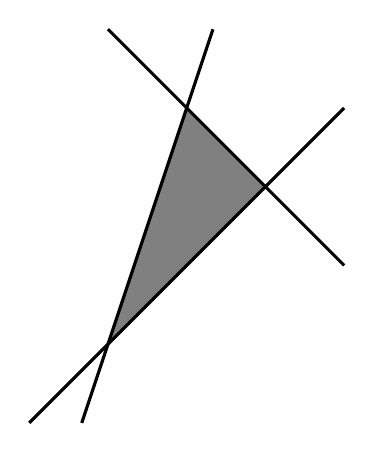
\begin{tikzpicture}
			\fill[gray] (0,1) -- (1,0) -- (-1,-2);
			\draw [line width=0.4mm] (-4/3,-3) -- (1/3,2);
			\draw [line width=0.4mm] (-1,2) -- (2,-1);
			\draw [line width=0.4mm] (-2,-3) -- (2,1);
		\end{tikzpicture}
		\end{center}
		\caption{An $\mathcal{H}$-polytope.}
		\label{fig:hpolytope}
		\end{figure}
		
		\emph{Now we will give the second definition of polytopes.}
		
		\definition{
			A \emph{$\mathcal{V}$-polytope} of dimension $d$ in $\mathbb{R}^n$ is the convex hull $P$ 
			(denoted $\text{conv}\{V\}$) of a finite set of points 
			$V \subset \mathbb{R}^n$ such that $P$ has affine span of dimension $d$.
		}
		
		The subset of points in $V$ on the boundary of the polytope is also called 
		the \emph{vertices} of the $\mathcal{V}$-polytope. 
		
		\example{
			The convex hull of the set of points $V = \{(0,1), (1,0), (-1,-2)\}$ create a $\mathcal{V}$-polytope. 
			See Figure \ref{fig:vpolytope} for a drawing of this polytope. 
		}
		
		\begin{figure}[H]
		\begin{center}
		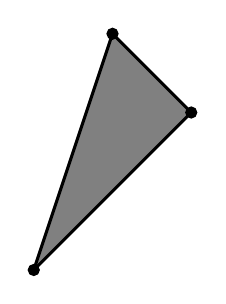
\begin{tikzpicture}
			\fill[gray] (0,1) -- (1,0) -- (-1,-2);
			\draw [line width=0.4mm] (0,1) -- (1,0);
			\draw [line width=0.4mm] (1,0) -- (-1,-2);
			\draw [line width=0.4mm] (-1,-2) -- (0,1);
			\draw (0,1)  circle[radius=2pt];
  			\fill (0,1)  circle[radius=2pt];
  			\draw (1,0)  circle[radius=2pt];
  			\fill (1,0)  circle[radius=2pt];
  			\draw (-1,-2)  circle[radius=2pt];
  			\fill (-1,-2)  circle[radius=2pt];
		\end{tikzpicture}
		\end{center}
		\caption{A $\mathcal{V}$-polytope.}
		\label{fig:vpolytope}
		\end{figure}
		
		\bigskip		
		
		\emph{As mentioned earlier, the set of $\mathcal{H}$-polytopes and the set of $\mathcal{V}$-polytopes are equal, as seen in the following theorem. }
		
		\theorem{ \label{thm:vhequality}
			Any $\mathcal{V}$-polytope is also an $\mathcal{H}$-polytope. Similarly, any $\mathcal{H}$-polytope is also a 
			$\mathcal{V}$-polytope.
		}
		\proof{
			Read Section \ref{proofHVequal}.
		}
		
		\example{
			The polytopes in Example 2.2 and Example 2.3 are in fact the same polytope.
		}
		
		\bigskip
		
		\emph{The boundaries of polytopes are themselves polytopes itself of smaller dimensions. 
		These are called \emph{faces} and are defined as follows. }
		
		\definition{
			A linear inequality $a \cdot x \leq b$, where $a\in \mathbb{R}^n,b\in \mathbb{R}$, is \emph{valid} for $P$ if it is satisfied for 
			all points $x\in P$. A \emph{face} of $P$ is any non-empty set of the form
			\[
			F = P \cap \{x\in \mathbb{R}^n:a \cdot x=b\}
			\]
			where $a \cdot x \leq b$ is a valid inequality for $P$. The \emph{dimension} of a face is the dimension of its affine span. 
		}
		
		\definition{
			Given a $d$-dimensional polytope $P$, the faces of dimension $d-1$ are called the \emph{facets} of $P$.
			Given a $d$-dimensional polytope $P$, the faces of dimension $1$ are called the \emph{edges} of $P$.
			Given a $d$-dimensional polytope $P$, the faces of dimension $0$ are called the \emph{vertices} of $P$.
		}
		
		\example{
			In Example 2.2, the hyperplanes are both the facets and the edges of the polytope, since the polytope is 
			2-dimensional and so the facets are 1-dimensional just like the edges. 
			The vertices of the polytope are the 3 points where the hyperplanes intersect.
		}
		
		\bigskip
		
		We end this part by naming polytopes where the vertices are integers.
		\definition{
			If $P = \text{conv}\{V\}$, where $V \subset \mathbb{Z}^n$, then $P$ is called a \emph{lattice polytope}.
		}
		
	\subsubsection{Proof of equality between $\mathcal{V}$-polytopes and $\mathcal{H}$-polytopes} \label{proofHVequal}
		We stated in Theorem \ref{thm:vhequality} that any $\mathcal{V}$-polytope is also 
		an $\mathcal{H}$-polytope, and any $\mathcal{H}$-polytope is also a $\mathcal{V}$-polytope. 
		In this section we prove this theorem. 
		The definitions, theorems, lemmas and proofs in this section are taken from 
		\cite{ZieglerLecturesOnPolytopes95}. 
		
		We start with some definitions. 
		
		\definition{
			A \emph{cone} is a non-empty set of vectors $C \subseteq \mathbb{R}^d$ that with any 
			finite set of vectors, also contains all their linear combinations with nonnegative 
			coefficients. In particular, every cone contains $\boldsymbol{0}$. 
		}
		
		\definition{
			For an arbitrary subset $Y \subseteq \mathbb{R}^d$ we define its \emph{conical hull} 
			cone$(Y)$ as the intersection of all cones in $\mathbb{R}^d$ that contains $Y$. 
			
			We define that cone$(Y) = \{ \boldsymbol{0} \}$ if $Y$ is the empty set.
		}
		
		\definition{
			The \emph{Minkowski sum} of two sets $P,Q \subseteq \mathbb{R}^d$ is defined to be 
			\[
			P + Q = \{ \boldsymbol{x} + \boldsymbol{y} : \boldsymbol{x} \in P, \boldsymbol{y} \in 
			Q\}.
			\]
		}
		
		\definition{
			An \emph{$\mathcal{H}$-polyhedron} denotes an intersection of closed halfspaces, 
			a set $P \subseteq \mathbb{R}^d$ presented in the form 
			\[
			P = P(A, \boldsymbol{z}) = \{\boldsymbol{x} \in \mathbb{R}^d : A\boldsymbol{x} \leq 
			\boldsymbol{z} \}
			\]
			for some $A \in \mathbb{R}^{m \times d}, \boldsymbol{z} \in \mathbb{R}^m$.
		}
		
		\definition{
			A \emph{$\mathcal{V}$-polyhedron} denotes any finitely generated convex-conical 
			combination: a set $P \subseteq \mathbb{R}^d$ that is given in the form 
			\[
			P = \text{conv}(V) + \text{cone}(Y)
			\]
			for some $V\in \mathbb{R}^{d \times n}, Y\in \mathbb{R}^{d \times n'}$, 
			as the Minkowski sum of a convex hull of a finite point set and the cone generated 
			by a finite set of vectors.
		}
		
		Now we can define a $\mathcal{V}$-polytope simply as a \emph{bounded} (contains no 
		ray $\{\boldsymbol{u} + t\boldsymbol{v} : t \geq 0, \boldsymbol{v} \neq 0\}$) 
		$\mathcal{V}$-polyhedron, and similary an $\mathcal{H}$-polytope is a bounded 
		$\mathcal{H}$-polyhedron. 
		
		Thus, Theorem \ref{thm:vhequality} follows if the theorem also is true for $\mathcal{H}$- 
		and $\mathcal{V}$-polyhedrons. 
		In order to prove that the theorem holds for polyhedrons, we first prove the case for 
		cones. 
		
		\theorem{ \label{thm:vhconeeq}
			A cone $C \subseteq \mathbb{R}^d$ is a finitely generated combination of vectors 
			(a \emph{$\mathcal{V}$-cone})
			\[
			C = \text{cone}(Y) \text{ for some } Y \in \mathbb{R}^{d \times n}
			\]
			if and only if it is a finite intersection of closed linear halfspaces 
			(an \emph{$\mathcal{H}$-cone})
			\[
			C = P(A, \boldsymbol{0}) \text{ for some } A\in \mathbb{R}^{m \times d}.
			\]
		}
		
		\emph{To prove Theorem \ref{thm:vhconeeq}, we need two lemmas, so we start by stating 
		and proving the lemmas.}
		
		\lemma{ \label{lemma:vtohcone}
			If $C=P(A, \boldsymbol{0})$ is an $\mathcal{H}$-cone in $\mathbb{R}^d$, then so is the 
			\emph{elimination} $\text{elim}_k (C) = \{ \boldsymbol{x} - t\boldsymbol{e}_k : 
			\boldsymbol{x} \in C, t\in \mathbb{R}\}$, and thus also the \emph{projection} 
			$\text{proj}_k(C) = \text{elim}_k (C)\cap H_k$ where $H_k = \{\boldsymbol{x} \in 
			\mathbb{R}^d : x_k = 0\}$ is a hyperplane. Namely, we get $\text{elim}_k (C) = 
			P(A^{/k}, \boldsymbol{0})$ for 
			\[
			A^{/k} = \{ \boldsymbol{a}_i : a_{ik}\} \cup \{a_{ik}\boldsymbol{a}_j + (-a_{jk}) 
			\boldsymbol{a}_ii : a_{ik} > 0, a_{jk} < 0 \}.
			\]
			(Here $A$ and $A^{/k}$ are interpreted as sets of row vectors.) 
		}
		
		\proof{
			We get that the row vectors in $A^{/k}$ are positive combinations of row vectors 
			in $A$, and as such are the corresponding inequalities in $C$ valid, so we get that 
			$C \subseteq P(A^{/k}, \boldsymbol{0})$. Also, the variable $x_k$ in the row 
			vectors of $A^{/k}$ does not appear in the system $A^{/k}\boldsymbol{x} \leq 
			\boldsymbol{0}$ since they are equal to zero by construction, which proves that 
			$\text{elim}_k (C) \subseteq P(A^{/k}, \boldsymbol{0})$. 
			
			Now for the converse, we let $\boldsymbol{x} \in P(A^{/k}, \boldsymbol{0})$ and 
			let $x_k = 0$. 
			We claim that $\boldsymbol{x} - y \boldsymbol{e}_k \in C$ for suitable $y$. 
			By using $\boldsymbol{x} - y \boldsymbol{e}_k$ in the system $A\boldsymbol{x} \leq 
			\boldsymbol{0}$, we find that $y$ has to satisfy 
			\[
			\max_i \left\{ \frac{1}{a_{ik}}\boldsymbol{a}_i \boldsymbol{x} : a_{ik} > 0\right\} 
			\leq y \leq \min_j \left\{ \frac{1}{-a_{jk}}(-\boldsymbol{a}_j)\boldsymbol{x} : a_{jk} 
			< 0 \right\}. 
			\]
			This is satisfied if $a_{ik} > 0$ and $a_{jk} < 0$, since then $\frac{1}{a_{ik}} 
			\boldsymbol{a}_i \boldsymbol{x} \leq \frac{1}{-a_{jk}} (-\boldsymbol{a}_j) 
			\boldsymbol{x}$. 
			This is equivalent to $(a_{ik}\boldsymbol{a}_j + (-a_{jk})\boldsymbol{a}_i)
			\boldsymbol{x} \leq 0$, which holds becase $\boldsymbol{x} \in P(A^{/k}, 
			\boldsymbol{0})$. $\blacksquare$
		}
		
		\lemma{ \label{lemma:htovcone}
			If $C = \text{cone}(Y)$ is a $\mathcal{V}$-cone in $\mathbb{R}^d$, then so is the 
			intersection $C\cap H_k$. Namely, we get $C\cap H_k = \text{cone}(Y^{/k})$ for 
			\[
			Y^{/k} = \{\boldsymbol{y}_i : y_{ki} = 0 \} \cup \{ y_{ki} \boldsymbol{y_j} + 
			(-y_{kj}) \boldsymbol{y}_i : y_{ki} > 0, y_{kj} < 0 \}. 
			\]
			(Here $Y$ and $Y^{/k}$ are interpreted as sets of columns vectors. Thus $y_{ki}$ 
			denotes the $k$th component of $\boldsymbol{y}_k$ and the $(k,i)$-entry of the 
			matrix $Y = (\boldsymbol{y}_1, ..., \boldsymbol{y}_n)$).
		}
		
		\proof{
			All the vectors in $Y^{/k}$ have $x_k = 0$, so $C \cap H_k \supseteq \text{cone}
			(Y^{/k})$. 
			
			For the reverse inclusion, consider some $\boldsymbol{v} = Y\boldsymbol{t} \in 
			\text{cone}(Y)$, where $\boldsymbol{t} \geq 0$ and $v_k = 0$. 
			Now we have $t_i y_{ki} = 0$ for all $i$ and we get $\boldsymbol{v} \in \text{cone} 
			( \{\boldsymbol{y}_i : y_{ki} = 0 \} )$, or we can expand $v_k = 0$ to get
			\[
			K = \sum_{i:y_{ki} > 0} t_i y_{ki} = \sum_{j:y_{kj} < 0} t_j(-y_{kj}) > 0.
			\]
			With this, we can rewrite $\boldsymbol{v}$ as 
			\begin{align*}
				\boldsymbol{v} &= 
				\sum_{i:y_{ki} = 0} t_i \boldsymbol{y}_i + 
				\sum_{i:y_{ki} > 0} t_i \boldsymbol{y}_i + 
				\sum_{j:y_{kj} < 0} t_j \boldsymbol{y}_j \\
				&= 
				\sum_{i:y_{ki} = 0} t_i \boldsymbol{y}_i + 
				\frac{1}{K} \sum_{i:y_{ki}>0} \left( \sum_{j:y_{kj}<0} t_j(-y_{kj}) \right) 
				t_i \boldsymbol{y}_i
				\frac{1}{K} \sum_{j:y_{kj}<0} \left( \sum_{i:y_{ki}<0} t_i y_{ki})
				\right) t_j \boldsymbol{y}_j \\
				&= 
				\sum_{i:y_{ki} = 0} t_i \boldsymbol{y}_i + 
				\sum_{\substack{i:y_{ki}>0 \\ j:y_{kj}<0}} \frac{t_i t_j}{K} \left(
				(-y_{kj})\boldsymbol{y}_j + y_{ki}\boldsymbol{y}_j \right).
			\end{align*}
			This gives an explicit representation of $\boldsymbol{v}$ as a conical sum of vectors 
			in $Y^{/k}$, which proves the lemma. $\blacksquare$
		}
		
		We are now prepared to prove Theorem \ref{thm:vhconeeq}. 
		
		\proof{ 
			For the direction from a $\mathcal{V}$-cone to an $\mathcal{H}$-cone, 
			let $C = \text{cone} (Y) \subseteq \mathbb{R}^d$ be a $\mathcal{V}$-cone. 
			We can write it as 
			\[
				C = \{Y \boldsymbol{t} \in \mathbb{R}^d : \boldsymbol{t} \geq \boldsymbol{0} \}
				= \{ \boldsymbol{x} \in \mathbb{R}^d : \exists \boldsymbol{t} \in \mathbb{R}^n : 
				\boldsymbol{t} \geq \boldsymbol{0}, \boldsymbol{x} = Y\boldsymbol{t} \}.
			\]
			Clearly, the set $\{(\boldsymbol{x},\boldsymbol{t}) \in \mathbb{R}^{d+n} : 
			\boldsymbol{t} \geq \boldsymbol{0}, \boldsymbol{x} = Y\boldsymbol{t} \}$ is an 
			$\mathcal{H}$-cone. Thus $C = \text{cone}(Y)$ can be written as the projection 
			of this cone to the subspace $\{(\boldsymbol{x},\boldsymbol{t}) \in \mathbb{R}^{d+n} : 
			\boldsymbol{t} = 0 \}$. 
			This projection can be formed successively, by projecting with respect to individual 
			$t_k$-coordinates one by one. This is proven in Lemma \ref{lemma:vtohcone}. 
			
			For the direction from an $\mathcal{H}$-cone to an $\mathcal{V}$-cone, 
			let $C = P(A,\boldsymbol{0}) \subseteq \mathbb{R}^d$ be an $\mathcal{H}$-cone. 
			We can write it as 
			\begin{align*}
				C &= \{ \boldsymbol{x} \in \mathbb{R}^d : A\boldsymbol{x} \leq \boldsymbol{0} \} \\
				&\cong \left\{ \left(\substack{\boldsymbol{x} \\ \boldsymbol{w}} \right) \in 
				\mathbb{R}^{d+m} : A\boldsymbol{x} \leq \boldsymbol{w} \right\} \cap 
				\left\{ \left(\substack{\boldsymbol{x} \\ \boldsymbol{w}} \right) \in 
				\mathbb{R}^{d+m} : \boldsymbol{w} = \boldsymbol{0} \right\}.
			\end{align*}
			Here, $\left\{ \left(\substack{\boldsymbol{x} \\ \boldsymbol{w}} \right) \in 
			\mathbb{R}^{d+m} : A\boldsymbol{x} \leq \boldsymbol{w} \right\}$ is a $\mathcal{V}$-
			cone, as shown above. 
			The intersection with $\left\{ \left(\substack{\boldsymbol{x} \\ \boldsymbol{w}} 
			\right) \in \mathbb{R}^{d+m} : \boldsymbol{w} = \boldsymbol{0} \right\}$ can be 
			formed successively, by setting coordinates to zero one at a time, i.e., intersecting 
			with coordinate hyperplanes of the form $H_k = \{ \boldsymbol{y} \in \mathbb{R}_{d+m} 
			: y_k = 0 \}$. This is proven in Lemma \ref{lemma:htovcone}. $\blacksquare$
		}
		
		We now present and prove the theorem for equality between $\mathcal{V}$-polyhedrons and 
		$\mathcal{H}$-polyhedrons. 
		
		\theorem{ \label{thm:hvpolyhedrons}
			A subset $P \subseteq \mathbb{R}^d$ is a sum of a convex hull of a finite set of points 
			plus a conical combination of vectors (a $\mathcal{V}$-polyhedron) 
			\[
			P = \text{conv}(V) + \text{cone}(Y) \text{ for some } V\in \mathbb{R}^{d \times n}, 
			Y \in \mathbb{R}^{d \times n}
			\]
			if and only if $P$ is an intersection of closed halfspaces (an $\mathcal{H}$-
			polyhedron)
			\[
			P = P(A, \boldsymbol{z}) \text{ for some } A\in \mathbb{R}^{m \times d}, 
			\boldsymbol{z} \in \mathbb{R}^m.
			\]
		}
		
		\proof{
			This theorem can be proven directly from Theorem \ref{thm:vhconeeq}. 
			To do this, we pass from affine $d$-space to linear $(d+1)$-space by adjoining an 
			extra coordinate (which is the zeroeth coordinate, note that every cone $C$ in Theorem 
			\ref{thm:vhconeeq}, by definition, contains the origin $\boldsymbol{0}$), 
			mapping the points $\boldsymbol{x} \in \mathbb{R}^d$ to the vector 
			$\left(\substack{1 \\ \boldsymbol{x}} \right) \in \mathbb{R}^{d+1}$. 
			This reduces this theorem to the special case where P is a cone. 
			
			To see this, we associate with every polyhedron $P \subseteq \mathbb{R}^d$ a cone 
			$C(P) \subseteq \mathbb{R}^{d+1}$ such that if $P = P (A, \boldsymbol{z})$ is an 
			$\mathcal{H}$-polyhedron, we define 
			\[
			C(P) = P \left( \left( \substack{-1 \\ -\boldsymbol{z}} \quad \substack{\mathbb{O} \\ 
			A} \right), \left( \substack{0 \\ \boldsymbol{0}} \right) \right).
			\]
			That is, if $P$ is defined by the inequalities $\boldsymbol{a}_i \boldsymbol{x} \leq 
			z_i$, then $C(P)$ is defined by the inequalities $-z_i x_+ \boldsymbol{a}_i 
			\boldsymbol{x} \leq 0$, together with the inequality $x_0 \geq 0$. 
			We see that $C(P)$ is again an $\mathcal{H}$-polyhedron in $\mathbb{R}^{d+1}$ and 
			\[
			P = \left\{ \boldsymbol{x} \in \mathbb{R}^d : \left( \substack{1 \\ \boldsymbol{x}} 
			\right) \in C(P) \right\}.
			\]
			Also, we see that if $P = P(B, \boldsymbol{u})$ is an arbitrary $\mathcal{H}$-
			polyhedron in $\mathbb{R}^{d+1}$, then $\{\boldsymbol{x} \in \mathbb{R}^{d} : 
			\left( \substack{1 \\ \boldsymbol{x}} \right) \in P \}$ is an $\mathcal{H}$-polyhedron 
			as well.
			
			If $P = \text{conv}(V) + \text{cone}(Y)$ is a $\mathcal{V}$-polyhedron, we define 
			\[
			C(P) = \text{cone} \left( \substack{\mathbbm{1} \\ V} \quad \substack{\mathbb{O} \\ Y} 
			\right).
			\]
			Then, $C(P)$ is again a $\mathcal{V}$-polyhedron in $\mathbb{R}^{d+1}$ and 
			\[
			P = \left\{ \boldsymbol{x} \in \mathbb{R}^d : \left( \substack{1 \\ \boldsymbol{x}} 
			\right) \in C(P) \right\}.
			\]
			Conversely, if $C = \text{cone}(W)$ is any cone in $\mathbb{R}^{d+1}$ generated by 
			vectors $\boldsymbol{w}_i$ with $w_{i0} \geq 0$, then $\{\boldsymbol{x} \in 
			\mathbb{R}^d : \left( \substack{1 \\ \boldsymbol{x}} \right) \in C \}$ is a 
			$\mathcal{V}$-polyhedron. 
			
			Now, given any $\mathcal{H}$-polyhedron $P$, we apply Theorem \ref{thm:vhconeeq} to 
			$C(P)$ to conclude that $C(P)$ is a $\mathcal{V}$-cone contained in $\{\boldsymbol{x} 
			\in \mathbb{R}^{d+1} : x_0 \geq 0 \}$, so $P$ is a $\mathcal{V}$-polytope as well. 
			Conversely, if $P$ is a $\mathcal{V}$-polyhedron, then accoring to Theorem 
			\ref{thm:vhconeeq} the associated cone $C(P)$ is a $\mathcal{H}$-polyhedron and so is 
			$P$. $\blacksquare$ 
		}
		
		We stated earlier that we can define aa $\mathcal{V}$-polytope 
		simply as a bounded $\mathcal{V}$-polyhedron, and similary an $\mathcal{H}$-polytope 
		is a bounded $\mathcal{H}$-polyhedron. 
		This means that we can apply Theorem \ref{thm:hvpolyhedrons} to polytopes, and 
		Theorem \ref{thm:vhequality} is thus proven.
		
\subsection{Ehrhart theory}
	
	\subsubsection{Rational generating functions}
		In order to introduce Ehrhart theory and Ehrhart polynomials, we first need a definition 
		and lemma about rational generating functions of a single variable, see \cite{braun2007ehrhart}.
		
		\definition{
			The \emph{generating function} for a sequence $\{a(k) : k\in \mathbb{Z}_{\geq 0} \}$ of 
			complex values is the power series 
			\[
			\sum_{k\in \mathbb{Z}_{\geq 0}} a(k)x^k \in \mathbb{C}[[x]].
			\]
		}
		
		A \emph{power series} is an infinite degree polynomial. 
		
		\lemma{ \label{lemma:ratgenfunc}
			A function $f(t) : \mathbb{C} \to \mathbb{C}$ is a polynomial of degree $d$ if and only 
			if there exists complex values $h_j^*$ such that 
			\[
			\frac{\sum_{j=0}^d h_j^*x^j}{(1-x)^{d+1}} = 
			\sum_{t\in \mathbb{Z}_{\geq 0}} f(t)x^t, \text{ and } 
			\sum_j h_j^* \neq 0.
			\]
		}
		
		\begin{proof}
			See Chapter 4 of \cite{StanleyEC1}.
		\end{proof}
		
		\emph{
		A consequence of Lemma \ref{lemma:ratgenfunc} is that if we have a polynomial $f(t)$ of 
		degree $d$ we can express it as 
		\[
		f(t) = \sum_{j=0}^d h_j^* \binom{t+d-j}{d},
		\]
		where $h_j^*$ are the coefficients in the numerator of the rational generating function 
		for $f(t)$. 
		}
		
		\example{
			If we let $f(t) = 2t^2 + 2t +1$, then 
			\begin{align*}
				\sum_{t\in \mathbb{Z}_{\geq 0}} f(t) x^t &= 
				2 \sum_{t\in \mathbb{Z}_{\geq 0}} t^2 x^t + 
				2 \sum_{t\in \mathbb{Z}_{\geq 0}} t x^t + 
				\sum_{t\in \mathbb{Z}_{\geq 0}} x^t \\
				&= 2 \left(x \frac{d}{dx} \right)^2 \sum_{t\in \mathbb{Z}_{\geq 0}} x^t
				+ 2 \left(x \frac{d}{dx} \right) \sum_{t\in \mathbb{Z}_{\geq 0}} x^t
				+ \sum_{t\in \mathbb{Z}_{\geq 0}} x^t \\ 
				&= 2 \left(x \frac{d}{dx} \right)^2 \frac{1}{1-x}
				+ 2 \left(x \frac{d}{dx} \right) \frac{1}{1-x}
				+ \frac{1}{1-x} \\ 
				&= \frac{2(x^2+x)}{(1-x)^3} + \frac{2(x-x^2)}{(1-x)^3} + \frac{(1-x)^2}{(1-x)^3} \\
				&= \frac{1 + 2x + x^2}{(1-x)^3}.
			\end{align*}
			Conversely,
			\begin{align*}
				\frac{1 + 2x + x^2}{(1-x)^3} &= (1 + 2x + x^2) \sum_{t\in \mathbb{Z}_{\geq 0}} 
				\binom{t+2}{2} x^t \\
				&= \sum_{t\in \mathbb{Z}_{\geq 0}} \left( \binom{t+2}{2} + 2 \binom{t+1}{2} 
				+ \binom{t}{2} \right) x^t \\ 
				&= \sum_{t\in \mathbb{Z}_{\geq 0}} \left(
				\frac{(t+2)(t+1)}{2} + \frac{2(t+1)t}{2} + \frac{t(t-1)}{2} \right) x^t \\ 
				&= \sum_{t\in \mathbb{Z}_{\geq 0}} (2t^2 + 2t + 1)x^t.
			\end{align*}
		}
		
	\subsubsection{Ehrhart polynomials}
	\emph{
		We introduce Ehrhart theory with lattice polytopes, using \cite{braun2007ehrhart} 
		as source.
	}
	
		\definition{
			For $P$, a lattice polytope in $\mathbb{R}^n$ of dimension $d$ and 
			set 
			\[
				L_p (t) := |tP \cap \mathbb{Z}^n|
			\] for $t \in \mathbb{Z}_{\geq 1}$. 
			The \emph{Ehrhart series of $P$} is 
			\[
				\text{Ehr}_p (x) := 1 + \sum_{t\in \mathbb{Z}_{\geq 1}} L_p (t) x^t.
			\]
		}
		
		\theorem{
			Let $P$, a lattice polytope in $\mathbb{R}^n$ of dimension $d$. 
			There exist complex values $h_j^*, 0 \leq j \leq d$, such that the Ehrhart 
			series for $P$ is a rational generating function of the following form:
			\[
				\text{Ehr}_p (x) = \frac{\sum_{j=0}^d h_j^* x^j}{(1-x)^{d+1}}, \quad
				\sum_j h_j^* \neq 0.
			\]
		}
		\proof{
			Check sources of dissertation for all proofs.
		}
		
		\corollary{ \label{col:lpt}
			$L_p (t)$ is expressible as a polynomial of degree $d$ in the variable $t$.
		}
		\proof{
			
		}
		
		\definition{
			The polynomial in Corollary \ref{col:lpt} is called the 
			\emph{Ehrhart polynomial} of $P$ and also denoted by $_p(t)$. The vector 
			$(h_0^*, h_1^*, ..., h_d^*)$ of coefficients of the numerator of 
			$\text{Ehr}_p(x)$ is called the \emph{$h$-star vector} for $P$.
		}
		
		\definition{
			Given a $d$-dimensional lattice polytope $P \subset \mathbb{R}^n$, 
			rhe \emph{relative volume} of a facet $F$ of $P$ is 
			\[
				\text{relvol}(F) := \lim_{t \ to \infty} \frac{1}{t^{d-1}} 
				|tF \cap \mathbb{Z}^n|.
			\]
		}
		
		\theorem{
			For any $d$-dimensional lattice polytope $P$, the $h^*$-vector of $P$ 
			satisfies $(h_0^*, ..., h_d^*) \in (\mathbb{Z}_{\geq 0})^{d+1}$. 
		}
		
		\proof{
			
		}
		
		\bigskip
		
		These definitions and theorems concern lattice polytopes, but it was shown in 
		\cite{Rassart2004} that polytopes not necessarily need to be lattice for there to exist 
		Ehrhart polynomials of the polytopes.